%!TEX root = ../thesis.tex
% ******************************* Thesis Appendix G ****************************
\chapter{Résumé étendu de la thèse}
\label{apx:G}
%*******************************************************************************
\selectlanguage{french}

%============================================================%
%============================================================%
\section{Introduction}
%============================================================%
%============================================================%

%============================================================%
\subsection*{Contexte industriel}
%============================================================%

%{\color{red} citer qq ref pour asseoir ce que tu dis sur le contexte}

L'enjeu actuel de la transition énergétique implique, entre autres, de réduire la part des énergies fossiles au sein du mix électrique mondial. 
Dans ce contexte, l'énergie éolienne en mer présente plusieurs avantages \cite{eolien_en_mer_2022}. 
L'éolien en mer bénéficie notamment de vents plus constants que l'éolien terrestre, notamment dû à l'absence de relief, et offre la possibilité d'installer des éoliennes plus grandes donc plus puissantes. 
Depuis l'installation de la première ferme éolienne en mer à Vindeby, au Danemark, en 1991, l'industrie a connu une croissance rapide, avec une capacité totale de 56 GW exploitée dans le monde en 2021. 
Au fil du temps, la technologie éolienne en mer s'est améliorée, aboutissant à des succès importants tels que la signature de projets non subventionnés en Europe (en anglais \textit{zero-subsidy bids}), pour lesquels l'électricité produite est directement vendue sur le marché de gros \cite{eolien_en_mer_2022}.

Cependant, malgré les progrès techniques indéniables, des limites industrielles émergent vis-à-vis de ces parcs éoliens en mer, posant ainsi de nombreux défis scientifiques. 
Pour atteindre les ambitieux objectifs de développement au niveau national et régional, la filière de l'éolien en mer fait face à plusieurs problèmes liés à l'augmentation de la taille des turbines.
Ce changement d'échelle crée notamment des tensions liées à la logistique portuaire, aux besoins en ressources primaires et à la gestion durable du démantèlement futur. 
Ce secteur présente plusieurs défis techniques et scientifiques, qui requièrent l'utilisation conjointe de données mesurées et de simulations numériques d'éoliennes dans leur environnement. 
La recherche appliquée à l'éolien en mer fait intervenir plusieurs disciplines qui étudient notamment des sujets tels que la conception d'éoliennes flottantes, l'amélioration de l'estimation des ressources éoliennes, l'optimisation des opérations de maintenance et l'augmentation de la durée de vie utile des parcs. 
De manière générale, plusieurs décisions sont prises durant la vie d'une éolienne par son concepteur, installateur et exploitant, tout en ayant une connaissance partielle de certains phénomènes physiques. 
Par conséquent, modéliser et maîtriser les diverses sources d'incertitudes associées à l'éolien en mer s'avère être un élément déterminant dans une industrie hautement concurrentielle.

Dans l'ensemble, l'industrie de l'éolien en mer a besoin de méthodes de traitement des incertitudes pour maîtriser les marges de sûreté et la gestion des actifs industriels (à la maille des composants, de l'éolienne et du parc dans son ensemble) \cite{OWT_review_2016}. 
Pour un développeur de projets éoliens, l'attention est d'abord portée sur l'amélioration du potentiel éolien des sites candidats en combinant différentes sources d'information et en modélisant la distribution multivariée des conditions environnementales au sein d'un parc éolien. 
Dans le cas de projets en éolien flottant, l'objectif est d'intégrer un aspect probabiliste dès la phase de conception (par exemple, du flotteur) afin de définir des solutions plus sûres, plus robustes et plus rentables. 
Pour un propriétaire d'un parc éolien, la gestion de la fin de vie est une autre problématique importante. 
Un propriétaire de parc éolien en fin de vie à le choix entre trois options : prolonger la durée de vie des actifs en exploitation, remplacer les éoliennes actuelles par des modèles plus récents, ou démanteler et vendre le parc éolien. 
Les deux premières solutions nécessitent d'évaluer la fiabilité de la structure et sa durée de vie résiduelle. Ces évaluations quantitatives sont examinées par des organismes de certification et des assureurs pour délivrer des permis d'exploitation. 
Pour fournir des évaluations rigoureuses des risques, la méthodologie générique de \textit{traitement des incertitudes} est une démarche qui fait consensus dans les secteurs industriels confrontés à ce genre de problématique \cite{rocquigny_2008}.


%============================================================%
\subsection*{Méthodologie générique de traitement des incertitudes dans les outils de calcul scientifiques}
%============================================================%

La simulation numérique est une discipline qui a émergé avec l'avènement de l'informatique. 
Cette pratique produit des outils de calcul scientifique (OCS) qui permettent de simuler le comportement de système complexes compte tenu de conditions initiales définies par l'analyste. 
Les OCS sont vite devenus indispensables pour l'analyse, la conception, et la certification de systèmes complexes dans les cas o\`u des expériences ou des mesures physiques sont coûteuses à obtenir, voire impossibles à réaliser. 
Cependant, ces modèles numériques s'intègrent dans une démarche déterministe : le résultat d'une simulation est associé à un vecteur de paramètres fixé en entrée. 
La question de la gestion des incertitudes associées aux entrées se pose rapidement lors de l'utilisation des OCS. 

Le traitement des incertitudes vise à modéliser et à traiter les incertitudes autour d'un modèle numérique. 
Pour ce faire, une méthodologie générique a été proposée pour quantifier et analyser les incertitudes entre les variables d'entrée et de sortie d'un OCS \cite{rocquigny_2008}. 
Une présentation des outils mathématiques utilisés dans ce domaine est proposée par \cite{sullivan_2015}.
Cette approche apporte une meilleure compréhension d'un système, ce qui contribue à une prise de décision plus robuste.   


La Figure \ref{fig:UQ_methodo} illustre les étapes génériques de la méthodologie de quantification des incertitudes, qui sont brièvement décrites ci-après :
\begin{itemize}
    \item[\textbullet] \textbf{\'Etape A -- Spécification du problème.} Cette étape consiste à déterminer le système étudié et construire un modèle numérique capable de simuler (précisément) son comportement. 
    La spécification du problème implique également de définir l'ensemble des paramètres inhérents au modèle numérique. 
    Ces paramètres comprennent aussi bien les variables d'entrée que les variables de sortie générées par la simulation. 
    Dans ce document, le modèle numérique est considéré comme une boîte-noire, par opposition à des approches qui s'intègrent à l'intérieur des schémas de résolution numérique des équations de comportement du système (approches dites intrusives \cite{lemaitre_2010}). 
    En général, ces modèles numériques sont au préalable calibrés par rapport à des données mesurées et suivent un processus de validation et de vérification pour réduire les erreurs de modélisation  \cite{oberkampf_2010_VVUQ}.
    \item[\textbullet] \textbf{\'Etape B -- Modélisation et quantification des incertitudes.} L'objectif de la deuxième étape est d'identifier et modéliser toutes les sources d'incertitude associées aux variables d'entrée. 
    Dans la plupart des cas, cette modélisation est effectuée dans un cadre probabiliste.
    \item[\textbullet] \textbf{\'Etape C -- Propagation des incertitudes.} Lors de cette étape, les entrées incertaines sont propagées au travers du modèle de simulation numérique. 
    Dès lors, la sortie du modèle numérique (habituellement de type scalaire) devient également incertaine. 
    L'objectif est alors d'estimer une quantité d'intérêt, c'est-à-dire une statistique sur la variable aléatoire de sortie étudiée. 
    La méthode de propagation de l'incertitude peut différer en fonction de la quantité d'intérêt visée (par exemple, la tendance centrale, un quantile, une probabilité d'événement rare, etc.). 
    \item[\textbullet] \textbf{\'Etape C' -- Analyse de sensibilité.} En complément de la propagation d'incertitudes, une analyse de sensibilité peut être réalisée afin d'étudier le rôle attribué à chaque entrée incertaine dans la variabilité de la sortie d'intérêt.
    %\vinc{Je casserai la liste ici, et je ferais une autre liste en précisant que, pour des raisons de coût calculatoire , etc, une étape de Métamodélisation peut être introduite afin de remplacer le code par un modèle de substitution (mais pour cela, il faut aussi faire A-B-C et même parfois C' pour réduire la dimension)}
    \item[\textbullet] \textbf{Métamodélisation.} Compte tenu du coût de calcul élevé que représentent certaines simulations, des approches statistiques visent à émuler ces simulateurs coûteux partir d'un nombre limité de simulations. 
    La quantification de l'incertitude peut alors être réalisée avec le modèle statique de substitution (ou métamodèle) pour un moindre coût de calcul. 
    Cette étape optionnelle d'apprentissage statistique ne fait pas à proprement dit partie du traitement des incertitudes mais elle s'avère souvent essentielle pour permettre sa mise en \oe uvre pratique. 
\end{itemize}

\begin{figure}[!h]
    \centering
    %\begin{figure}[h]
%    \centering
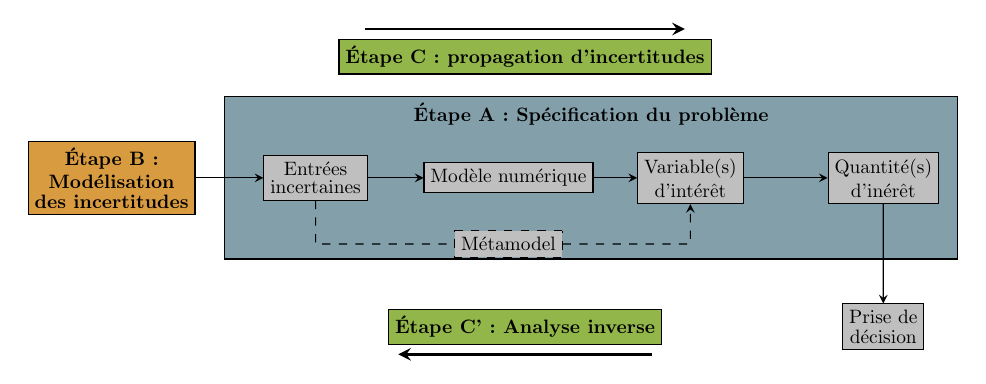
\begin{tikzpicture}[scale=0.7, every node/.style={transform shape}]
    \node[rectangle,draw,fill=YellowOrange!70!gray] (a) at (-9,0) {\shortstack{\textbf{\'Etape B :} \\ \textbf{Mod\'{e}lisation} \\ \textbf{des incertitudes}}};
\node[rectangle,draw,fill=YellowGreen!70!gray] (f) at (-1.5,2.2) {
\textbf{\'Etape C : propagation d'incertitudes}};
\node[rectangle,draw,fill=YellowGreen!70!gray] (g) at (-1.5,-2.7) {\shortstack{
\textbf{\'Etape C' : Analyse inverse}}};
\node[rectangle,draw,minimum width=13.3cm,fill=SkyBlue!40!gray] (h) at (-0.3,0) {\shortstack{\textbf{\'Etape A : Sp\'{e}cification du problème} \\ \phantom{a} \\ \phantom{a} \\ \phantom{a} \\ \phantom{a} \\ \phantom{a} \\ \phantom{a} \\ \phantom{a} \\ \phantom{a} \\ \phantom{a} }};
\node[rectangle,draw,fill=lightgray] (b) at (-5.3,0) {\shortstack{
Entr\'{e}es\\ incertaines}};
\node[rectangle,draw,fill=lightgray] (c) at (-1.8,0) {\shortstack{
    Modèle num\'{e}rique}};
\node[rectangle,draw,fill=lightgray] (d) at (1.5,0) {\shortstack{
Variable(s) \\ d'int\'{e}rêt}};
\node[rectangle,draw,fill=lightgray] (e) at (5,0) {\shortstack{
Quantit\'{e}(s) \\ d'in\'{e}rêt}};
\node[rectangle,draw,fill=lightgray, dashed] (i) at (-1.8,-1.2) {M\'{e}tamodel};
\node[rectangle,draw,fill=lightgray] (j) at (5,-2.7) {\shortstack{Prise de \\ d\'{e}cision}};
\draw[-stealth, black, line width=1pt] (-4.4,2.7) -- (1.4,2.7);
\draw[-stealth, black, line width=1pt] (0.8,-3.2) -- (-3.8,-3.2);
\draw[-stealth, black] (a) -- (b);
\draw[-stealth, black] (b) -- (c);
\draw[-stealth, black] (c) -- (d);
\draw[-stealth, black] (d) -- (e);
\draw[-stealth, black, dashed] (b) -- (-5.3,-1.2) -- (i) -- (1.5,-1.2) -- (d);
 \draw[-stealth, black] (e) -- (j);

\end{tikzpicture}
%    \caption{General uncertainty quantification and propagation framework}
%    \label{Fig:UQ}
%\end{figure}
    \caption{Schéma générique de la quantification des incertitudes (\cite{rocquigny_2008}, adapté par \cite{ajenjo_2023})}
    \label{fig:UQ_methodo_FR}
\end{figure}


%============================================================%
\subsection*{Verrous scientifiques et objectifs de la thèse}
%============================================================%

La maîtrise des risques et des incertitudes dans l'éolien est un enjeu majeur pour le groupe EDF en tant qu'exploitant. 
Cette thèse vise à adapter et appliquer, sur un cas d'usage issu de l'éolien en mer, une démarche globale de traitement des incertitudes. 
Ainsi, ce cas d'usage soulève des verrous scientifiques associés à ses particularités qui peuvent être décrites comme suit :
\begin{itemize}
    \item[\textbullet] Le code de simulation numérique autour duquel les travaux sont réalisés est constitué d'une chaîne de codes de calcul, exécutés en série. 
    Cette chaîne s'articule en trois étapes: d'abord une génération temporelle et stochastique d'un champ de vitesse de vent et de houle, puis la simulation du comportement hydro-aéro-servo-élastique de l'éolienne et enfin une phase d'agrégation des résultats temporels pour obtenir des quantités d'intérêt scalaires ;
    \item[\textbullet] La complexité de cet outil de calcul scientifique ainsi que le coût de calcul unitaire élevé (de l'ordre de 20 minutes par simulation) nécessite l'utilisation de méthodes d'échantillonage performantes, ainsi que des systèmes de calcul haute performance. 
    En plus de la complexité liée au modèle numérique, la modélisation des incertitudes en entrée présente elle aussi des difficultés. 
    En effet, la loi conjointe des conditions environnementales liées à un site comporte une structure de dépendance complexe à capturer et à modéliser. 
    L'étape d'inférence vis-à-vis des grandes quantités de données mesurées est d'autant plus importante que sa qualité impacte directement les conclusions de la propagation d'incertitudes.
\end{itemize}

Afin d'appliquer le schéma global de traitement des incertitudes au cas éolien, cette thèse vise à répondre aux problématiques suivantes:
\begin{itemize}
    \item[\textbf{Q1.}] \textit{
    Comment précisément modéliser la structure de dépendance complexe associée aux lois conjointes de conditions environnementales ?
    } (\ding{238} \'Etape B)
    \item[\textbf{Q2.}] \textit{
    Comment réaliser une propagation d'incertitudes au travers d'une chaîne de simulation numérique coûteuse, uniquement basée sur une description empirique (données mesurées) des incertitudes en entrée ?
    } (\ding{238} \'Etape C)
    \item[\textbf{Q3.}] \textit{
    Comment estimer des probabilités d'événements rares associées à la ruine de structures éoliennes en mer ?
    } (\ding{238} \'Etape C)
    \item[\textbf{Q4.}] \textit{
    Comment évaluer et interpréter la sensibilité des entrées incertaines vis-à-vis des quantités d'intérêt liées à la fiabilité des structures (analyse de sensibilité fiabiliste) ?
    } (\ding{238} \'Etape C')
\end{itemize}
Les sections suivantes résument les travaux de thèse, tout en respectant la structure du manuscrit. 



%============================================================%
%============================================================%
\section{Résumés des chapitres relatifs à l'état de l'art des méthodes et outils mis en \oe{}uvre dans la thèse}
%============================================================%
%============================================================%


Les deux premiers chapitres relaterons l'état de l'art dans le domaine du traitement des incertitudes et de la modélisation numérique des systèmes éoliens. 

%------------------------------------------------------------%
\subsection*{Chapitre 1 -- Traitement des incertitudes en simulation numérique}
%------------------------------------------------------------%
Ce chapitre vise à présenter un état de l'art concis des différentes thématiques en quantification des incertitudes \cite{sullivan_2015}. 
Après un rappel de quelques prérequis mathématiques, l'étape de spécification du modèle numérique (considéré comme étant une boîte-noire), ainsi que les variables d'entrée et de sortie est détaillée. 
Les différents types et sources d'incertitudes sont ensuite présentés, ainsi que leur modélisation dans un cadre probabiliste. 
La propagation des incertitudes dépend de la nature des quantités d'intérêt estimées, ainsi, une section aborde les méthodes de propagation pour l'étude en tendance centrale et une autre s'intéresse aux problèmes d'estimation de probabilités d'événements rares (statistiques liées aux queues de distributions). 
La section dédiée à la tendance centrale présente des méthodes d'intégration numérique, d'échantillonage et de planification d'expériences \cite{fang_liu_2018}. 
Celle consacrée aux probabilités d'événements rares présente des méthodes classiques issues du domaine de la fiabilité des structures \cite{ lemaire_2013,MorioBalesdent2015}.

Ce chapitre aborde également les principales méthodes d'analyse de sensibilité globale \cite{daveiga_iooss_2021}. 
Ce domaine divise ses méthodes en deux grandes classes : les méthodes de criblage et les mesures d'importance. 
D'une part, les techniques de criblage, généralement mises en \oe{}uvre dans les problèmes de grande dimension, visent à identifier les variables n'ayant qu'un faible impact sur la variabilité de la sortie d'intérêt. 
D'autre part, les mesures d'importances visent, quant à elles, à attribuer de manière quantitative, pour chaque variable d'entrée, une part de variabilité de la sortie, permettant de proposer un classement des variables en fonction de leur influence.

Finalement, ce chapitre présente un panorama des familles de métamodèles communément utilisés en quantification des incertitudes \cite{forrester_2008}. 
Une attention particulière est apportée à la régression par processus gaussiens qui revient à conditionner un processus gaussien par un ensemble d'observations du code de simulation numérique. 
Une fois conditionné, le processus gaussien apporte une information plus riche que d'autres types de métamodèles. 
En effet, cette méthode propose conjointement un métamodèle (un prédicteur, ou moyenne du processus), et une fonction d'erreur (variance du processus). 
Certaines méthode itératives (dites \og actives \fg{}) exploitent cette information complémentaire pour enrichir progressivement le métamodèle et améliorer sa prédictivité. 
Ces techniques ont connu un franc succès dans les années 90 pour résoudre des problèmes d'optimisation de fonctions coûteuses \cite{jones_1998}. 
Depuis, leur utilisation s'est étendue à la résolution de problèmes de fiabilité des structures \cite{echard_2011}.

%------------------------------------------------------------%
\subsection*{Chapitre 2 -- Introduction à la modélisation et la conception de systèmes éoliens}
%------------------------------------------------------------%

La simulation d'une éolienne en mer implique la modélisation de plusieurs physiques en interaction avec des conditions environnementales de nature aléatoire. 
Ce chapitre introduit premièrement les méthodes spectrales utilisées pour générer des champs de vitesse de vent et de houle en appliquant des transformées de Fourier inverses (par exemple implémentées dans l'outil TurbSim \cite{turbsim_2009}). 
Ces champs de vitesses de vent simulés alimentent par la suite un outil de simulation multi-physique des éoliennes. 
Cette simulation intègre une modélisation simplifiée des interactions entre fluides et structures (méthode "BEMT" pour \textit{blade element momentum theory}), une modélisation dynamique de la structure par des éléments finis de type poutre, et une modélisation du contrôle-commande de l'éolienne \cite{milano_thesis_2021}. 
Ce code numérique produit en sortie des séries temporelles de plusieurs grandeurs physiques décrivant le comportement du système.

Cette thèse s'intéresse particulièrement à l'évaluation probabiliste du dommage en fatigue des structures éoliennes. 
Le dommage en fatigue est un phénomène qui détériore les propriétés mécaniques d'un matériau suite à sa sollicitation via un grand nombre de contraintes cycliques de faible amplitude. 
A l'heure actuelle, les standards \cite{iec_2019,dnv_loads_2016} recommandent l'utilisation de coefficients de sécurité déterministes pour faire face à ce mode de défaillance. 
Une approche probabiliste permet d'enrichir l'analyse et parfois de mettre en évidence le conservatisme des marges de sûreté. 
Plusieurs travaux récents se sont intéressés à cette thématique en abordant des angles méthodologiques différents \cite{huchet_2019,lataniotis_2019,cousin_2021,hirvoas_2021,petrovska_2022}.

Dans ce contexte, ce chapitre liste les paramètre d'entrée de la chaîne de calcul considérés comme incertains par la suite. 
Ces variables aléatoires sont regroupées en deux groupes : le vecteur aléatoire lié à l'environnement (par exemple : la vitesse moyenne du vent, l'écart-type de la vitesse du vent, la direction du vent, la hauteur de houle, la période de houle, et la direction de houle), et le vecteur aléatoire lié au système (par exemple : l'erreur de d'alignement au vent du contrôleur, la rigidité du sol, les paramètres des courbes de calcul de fatigue).


%============================================================%
%============================================================%
\section{Résumés des chapitres relatifs aux contributions méthodologiques et apports vis-à-vis des applications}
%============================================================%
%============================================================%

Après avoir dressé l'état de l'art sur ce sujet, les prochains chapitres du manuscrit présentent les nouvelles contributions de la thèse. 
D'un point de vue méthodologique, un objet mathématique servira de fil conducteur au cours de ces travaux. 
La \textit{maximum mean discrepancy} (MMD) \cite{oates_21} est une measure de dissimilarité entre des lois de probabilité basée sur des noyaux qui est utilisée dans des contextes différents (tests statistiques \cite{gretton_2006}, analyse de sensibilité \cite{daveiga_2015}, échantillonage \cite{pronzato_zhigljavsky_2020}, etc.).

%------------------------------------------------------------%
\subsection*{Chapitre 3 -- Quantification des perturbations induites par les effets de sillage au sein d'un parc éolien}
%------------------------------------------------------------%

Ce chapitre étudie les perturbations sur les conditions environnementales à l'intérieur d'une ferme éolienne en mer induites par les effets de sillage (\textit{wake effect} en anglais) \cite{larsen_2008_wake}. 
Un parc éolien en mer théorique au large de la côte sud de la Bretagne est considéré comme cas d'usage, et un modèle numérique simulant le sillage de ce parc est exploité. 
Ce modèle donne une prédiction analytique du déficit en vitesse de vent et de la turbulence créés par le sillage, en tenant compte de l'influence de la position des flotteurs en raison des forces moyennes du vent. 
Une propagation de l'incertitude sur le modèle de sillage est réalisée, en considérant la loi conjointe des conditions environnementales ambiantes en entrée. 
Au final une distribution environnementale perturbée par le sillage est simulée pour chaque éolienne. 
Une mesure de dissimilarité (la MMD) est utilisée pour comparer les distributions perçues par chaque éolienne. 
Cette quantité permet de regrouper les éoliennes (phase de \textit{clustering}) exposées à des conditions environnementales similaires, entraînant une réponse structurelle identiques. 
Compte tenu du coût de calcul élevé des simulations aéro-servo-hydro-élastiques des éoliennes en mer, cette étude préalable permet de réaliser une analyse de fiabilité à l'échelle d'une ferme éolienne sans répéter l'analyse pour chaque turbine. 
En fin de compte, seules quatre classes sont retenues pour représenter une ferme de 25 éoliennes. 
Ce travail a mené à la publication suivante : \\

\noindent
\ding{43} A. Lovera, \underline{E. Fekhari}, B. Jézéquel, M. Dupoiron, M. Guiton and E. Ardillon (2023). ``Quantifying and clustering the wake-induced perturbations within a wind farm for load analysis". In: \textit{Journal of Physics: Conference Series (WAKE 2023)}, Visby, Sweden. 

%------------------------------------------------------------%
\subsection*{Chapitre 4 -- Méthodes à noyaux pour l'estimation de la tendance centrale}
%------------------------------------------------------------%

Ce chapitre présente une utilisation d'une mesure de dissimilarité basée sur des noyaux (la MMD) pour échantillonner suivant une loi de probabilité, méthode du ``\textit{kernel herding}'' introduite par \cite{chen_welling_2010}. 
Cette technique de quadrature appartient à la famille dite des \og quadratures Bayésiennes \fg{} \cite{briol_oates_2019} qui s'interprètent comme une généralisation des méthodes de quasi-Monte Carlo \cite{hickernell_2020}. 
Le \textit{kernel herding} est présenté en détails et plusieurs expériences numériques sur des fonctions analytiques illustrent son intérêt. 

Les propriétés de cette méthode sont mises en valeur via une application industrielle dédiée à l'estimation de la moyenne du dommage en fatigue d'une structure éolienne. 
Cette quantité est déterminante dans le dimensionnement et la certification des éoliennes. 
Toutefois, son estimation par le biais de simulations numériques s'avère coûteuse. 
L'étude est réalisée sur un modèle d'une éolienne posée appartenant à une ferme installée en mer du Nord. 
Les incertitudes des conditions environnementales en entrée sont inférées sur des données mesurées in-situ. 

Dans ce cadre, une comparaison numérique avec un échantillonnage Monte Carlo et quasi-Monte Carlo révèle la performance et les avantages pratiques du \textit{kernel herding}.
Cette méthode permet notamment sous-échantillonner directement depuis une base de données environnementales importante, sans effectuer d'inférence (étape B). 
Ce travail a mené à la publication et au développement informatique suivant : \\

\noindent
\ding{43} \underline{E. Fekhari}, V. Chabridon, J. Muré and B. Iooss (2023). ``Given-data probabilistic fatigue assessment for offshore wind turbines using Bayesian quadrature''. In: \textit{Data-Centric Engineering}, In press.\\

\noindent
\ding{43} Le module Python \href{https://github.com/efekhari27/ctbenchmark}{\texttt{ctbenchmark}} standardise les expériences numériques liées à la quadrature Bayésienne et est disponible sur la plateforme GitHub.\\

\noindent
\ding{43} Le module Python \href{https://github.com/efekhari27/copulogr    m}{\texttt{copulogram}} propose une nouvelle représentation graphique de jeux de données multivariés et est disponible sur la plateforme de téléchargement Pypi.



%------------------------------------------------------------%
\subsection*{Chapitre 5 -- Méthodes à noyaux pour la validation de métamodèles}
%------------------------------------------------------------%

Ce chapitre propose une utilisation des méthodes d'échantillonage à base de noyaux dans le cadre de la validation de modèles d'apprentissage (ou métamodèles). 
L'estimation de la prédictivité des modèles d'apprentissage supervisé nécessite une évaluation de la fonction apprise sur un ensemble de points de test (non utilisés par lors de l'apprentissage). 
La qualité de l'évaluation dépend naturellement des propriétés de l'ensemble de test et de la statistique d'erreur utilisée pour estimer l'erreur de prédiction. 
Cette contribution propose d'une part d'utiliser des méthodes d'échantillonage pour sélectionner de manière ``optimale'' un ensemble de test et d'autre part présente un nouveau critère de prédictivité qui pondère les erreurs observées pour obtenir une estimation globale de l'erreur. 
Une comparaison numérique entre plusieurs méthodes d'échantillonage basées sur des approches géométriques \cite{shang_apley_2020} ou sur des méthodes à noyaux \cite{chen_welling_2010,mak_joseph_2018} est effectuée. 
Nos résultats montrent que les versions pondérées des méthodes à noyau offrent des performances supérieures. 
Une application aux efforts mécaniques simulées par un modèle éolien en mer est également présentée. 
Cette expérience illustre la pertinence pratique de cette technique comme alternative efficace aux techniques coûteuses de validation croisée. 
Ce travail a mené à la publication et au développement informatique suivant : \\

\noindent
\ding{43} \underline{E. Fekhari}, B. Iooss, J. Muré, L. Pronzato and M.J. Rendas (2023). ``Model predictivity assessment: incremental test-set selection and accuracy evaluation''. In: \textit{Studies in Theoretical and Applied Statistics}, pages 315--347. Springer.\\

\noindent
\ding{43} Le module Python \href{https://efekhari27.github.io/otkerneldesign/master/}{\texttt{otkerneldesign}} est développé en collaboration avec J.Muré. Ce module dédié à la quadrature Bayésienne est documenté et disponible sur la plateforme de téléchargement Pypi. 


%------------------------------------------------------------%
\subsection*{Chapitre 6 -- Estimation non-paramétrique de probabilités d'événements rares \label{sec:chap6}}
%------------------------------------------------------------%

L'estimation de probabilités d'événements rares est un problème courant dans la gestion des risques industriels, notamment dans le domaine de la fiabilité des structures \cite{chabridon_2018_thesis}. 
Pour ce faire, plusieurs techniques ont été proposées pour surmonter les limites connues de la méthode de Monte Carlo. 
Parmi elles, la méthode de ``\textit{subset sampling}'' \cite{AuBeck2001} est une technique qui repose sur la décomposition de la probabilité de l'événement rare en un produit de probabilités conditionnelles moins rares (donc plus simples à estimer) associées à des événements de défaillance imbriqués. 
Cependant, cette technique repose sur la simulation conditionnelle à base de méthodes de Monte Carlo par chaînes de Markov (MCMC). 
Ces algorithmes permettent, à la convergence, de simuler selon la densité cible. 
Cependant, en pratique, ils produisent souvent des échantillons non indépendants et identiquement distribués (i.i.d.) en raison de la corrélation entre les chaînes de Markov. 
Ce chapitre propose une autre méthode pour échantillonner conditionnellement aux événements de défaillance imbriqués afin d'obtenir des échantillons dont la propriété d'être i.i.d. est préservée. 
La propriété d'indépendance des échantillons est particulièrement pertinente pour exploiter ces mêmes échantillons pour une analyse de sensibilité fiabiliste. 
L'algorithme proposé repose sur l'inférence non-paramétrique de la distribution conjointe conditionnelle en utilisant une estimation par noyau des marginales combinée à une inférence de la dépendance à l'aide de la copule empirique de Bernstein \cite{sancetta_satchell_2004}. 
L'algorithme appelé \textit{``Bernstein adaptive nonparametric conditional sampling''} (BANCS) est comparée à la méthode du \textit{subset sampling} pour plusieurs problèmes de fiabilité des structures. 
Les premiers résultats sont encourageants, mais le contrôle du biais de l'estimateur doit être plus amplement investigué. 
Ce travail a mené à la publication et au développement informatique suivant : \\

\noindent
\ding{43} \underline{E. Fekhari}, V. Chabridon, J. Muré and B. Iooss (2023). ``Bernstein adaptive nonparametric conditional sampling: a new method for rare event probability estimation''. In: \textit{Proceedings of the 13th International Conference on Applications of Statistics and Probability in Civil Engineering (ICASP 14)}, Dublin, Ireland.\\

\noindent
\ding{43} Le module Python \href{https://github.com/efekhari27/bancs}{\texttt{bancs}} propose une implémentation de la méthode BANCS et est disponible sur la plateforme GitHub. 

%------------------------------------------------------------%
\subsection*{Chapitre 7 -- Analyse de sensibilité fiabiliste adaptative}
%------------------------------------------------------------%

Ce chapitre traite d'analyse de sensibilité pour des mesures de risque (par exemple, un probabilité d'événement rare). 
L'analyse de sensibilité globale \cite{daveiga_iooss_2021} attribue à chaque variable (ou groupe de variable) une part de variabilité globale de la sortie (le plus souvent à l'aide d'une décomposition fonctionnelle de la variance de la sortie). 
Cependant, les variables ayant un impact sur des quantités liées à une queue de distribution peuvent être très différentes que celles ayant un impact sur la variabilité globale (pondérée par le poids associé au centre de la distribution). 
L'analyse de sensibilité fiabiliste (en anglais ``\textit{reliability-oriented sensitivity analysis}'', \cite{chabridon_2018_thesis}) permet d'expliquer le rôle des entrées vis-à-vis de probabilités d'événements rares. 
L'idée de ce chapitre est d'étudier l'évolution de la sensibilité au fur et a mesure que l'échantillonnage se rapproche de l'événement rare. 
Cette analyse permet ainsi d'exploiter les paquets successifs d'échantillons conditionnels générés par l'algorithme BANCS (présenté dans le Chapitre 6). 
En post-traitement de l'estimation de la probabilité d'un événement rare, cette approche utilise une mesure d'importance à base de noyaux, nommée \textit{Hilbert-Schmidt Indepencence Criterion}, pour évaluer la dynamique de la sensibilité fiabiliste \cite{marrel_chabridon_2021}.

%============================================================%
%============================================================%
\section{Conclusion}
%============================================================%
%============================================================%

En résumé, cette thèse aborde plusieurs aspects du traitement des incertitudes à l'aide d'outils mathématiques à base de noyaux et présente un débouché industriel lié à l'enjeu de la maîtrise des risques des actifs éoliens en mer. Les contributions de cette thèse ont été principalement réalisées dans le cadre du projet européen HIPERWIND (\textit{HIghly advanced Probabilistic design and Enhanced Reliability methods for high-value, cost-efficient offshore wind.}), et de l'ANR INDEX (INcremental Design of EXperiments). Le sous-sections ci-après résument les communications, les publications dans revue à comité de lecture et les développements informatiques.

\subsection{Communications et publications dans revues à comité de lecture}

\begin{center}
    \footnotesize
    \renewcommand*{\arraystretch}{1.4}
    \begin{tabularx}{\textwidth}{l X}
        Book Chap. & \underline{E. Fekhari}, B. Iooss, J. Muré, L. Pronzato and M.J. Rendas (2023). 
                    ``Model predictivity assessment: incremental test-set selection and accuracy evaluation''. 
                    In: \textit{Studies in Theoretical and Applied Statistics}, pages 315--347. Springer.\\
        \hline
        Jour. Pap.   & \underline{E. Fekhari}, V. Chabridon, J. Muré and B. Iooss (2023).
                    ``Given-data probabilistic fatigue assessment for offshore wind turbines using Bayesian quadrature''. 
                    In: \textit{Data-Centric Engineering}, In press.\\
        \hline
        Int. Conf   & \underline{E. Fekhari}, B. Iooss, V. Chabridon, J. Muré (2022).
                    ``Numerical Studies of Bayesian Quadrature Applied to Offshore Wind Turbine Load Estimation''.
                    In: \textit{SIAM Conference on Uncertainty Quantification (SIAM UQ22)}, Atlanta, USA. (Talk)\\
        
                    & \underline{E. Fekhari}, B. Iooss, V. Chabridon, J. Muré (2022). 
                    ``Model predictivity assessment: incremental test-set selection and accuracy evaluation''.
                    In: \textit{22nd Annual Conference of the European Network for Business and Industrial Statistics (ENBIS 2022)}, Trondheim, Norway. (Talk)\\
        
                    & \underline{E. Fekhari}, B. Iooss, V. Chabridon, J. Muré (2022). 
                    ``Efficient techniques for fast uncertainty propagation in an offshore wind turbine multi-physics simulation tool''.
                    In: \textit{Proceedings of the 5th International Conference on Renewable Energies Offshore (RENEW 2022)}, Lisbon, Portugal. (Paper \& Talk)\\
        
                    & \underline{E. Fekhari}, V. Chabridon, J. Muré and B. Iooss (2023). 
                    ``Bernstein adaptive nonparametric conditional sampling: a new method for rare event probability estimation''\footnote{Cette contribution a été récompensée par le ``CERRA Student Recognition Award''}.
                    In: \textit{Proceedings of the 13th International Conference on Applications of Statistics and Probability in Civil Engineering (ICASP 14)}, Dublin, Ireland. (Paper \& Talk)\\
        
                    & E. Vanem, \underline{E. Fekhari}, N. Dimitrov, M. Kelly, A. Cousin and M. Guiton (2023). 
                    ``A joint probability distribution model for multivariate wind and wave conditions''.
                    In: \textit{Proceedings of the ASME 2023 42th International Conference on Ocean, Offshore and Arctic Engineering (OMAE 2023)}, Melbourne, Australia. (Paper)\\
        
                    & A. Lovera, \underline{E. Fekhari}, B. Jézéquel, M. Dupoiron, M. Guiton and E. Ardillon (2023). 
                    ``Quantifying and clustering the wake-induced perturbations within a wind farm for load analysis". 
                    In: \textit{Journal of Physics: Conference Series (WAKE 2023)}, Visby, Sweden (Paper)\\
        \hline
        Nat. Conf.  & \underline{E. Fekhari}, B. Iooss, V. Chabridon, J. Muré (2022).
                    ``Kernel-based quadrature applied to offshore wind turbine damage estimation''. 
                    In: \textit{Proceedings of the Mascot-Num 2022 Annual Conference (MASCOT NUM 2022)}, Clermont-Ferrand, France (Poster)\\
        
                    & \underline{E. Fekhari}, B. Iooss, V. Chabridon, J. Muré (2023).
                    ``Rare event estimation using nonparametric Bernstein adaptive sampling''. 
                    In: \textit{Proceedings of the Mascot-Num 2023 Annual Conference (MASCOT-NUM 2023)}, Le Croisic, France (Talk)\\
                    
        \end{tabularx}
\end{center}

\newpage
\subsection{Développements informatiques open source}

\texttt{otkerneldesign}\footnote{Documentation:\url{https://efekhari27.github.io/otkerneldesign/master/}}
\begin{itemize}
    \item[\textbullet] Ce module Python génère des échantillons (aussi appelés plans d'expérience) en utilisant des méthodes à base de noyaux comme le \textit{kernel herding} et les \textit{support points}. Une implementation tensorisée qui améliore grandement les performances est également proposée. En complément, une méthode de pondération ``optimale'' à l'aide de quadrature Bayésienne est proposée. 
    \item[\textbullet] Ce module est développé en collaboration avec J. Muré, est documenté et disponible sur la plateforme de téléchargement Pypi.
\end{itemize}

\texttt{bancs\footnote{Dépôt: \url{https://github.com/efekhari27/bancs}}}     
\begin{itemize}
    \item[\textbullet] Ce module Python offre une implémentation de la méthode ``\textit{Bernstein Adaptive Nonparametric Conditional Sampling}'' mentionnée en Section \ref{sec:chap6}. 
    \item[\textbullet] Ce module est disponible sur la plateforme de GitHub et son utilisation est illustrée par des exemples analytiques.
\end{itemize}

\texttt{ctbenchmark\footnote{Repository: \url{https://github.com/efekhari27/ctbenchmark}}}    
\begin{itemize}
    \item[\textbullet] Ce module Python standardise les comparaisons numériques réalisés pour étudier les méthodes de quadrature Bayésiennes.      
    \item[\textbullet] Le module et les expériences numériques sont disponibles sur un dépôt GitHub.
\end{itemize}

\texttt{copulogram\footnote{Repository: \url{https://github.com/efekhari27/copulogram}}} 
\begin{itemize}
    \item[\textbullet] Ce module Python propose une nouvelle représentation graphique de jeux de données multivariés appelée \textit{copulogram}.
    \item[\textbullet] Ce module, développé en collaboration avec V. Chabridon, est disponible sur la plateforme de téléchargement Pypi.
\end{itemize}
